% Auto-generated LaTeX figure includes

% Figure 1: Radar profiles
\begin{figure}[t]
  \centering
  
\includegraphics[width=0.45\textwidth]{figures/fig1_radar_profiles.pdf}
  \caption{Response style profiles across 8 psychometric dimensions for selected models (gray: remaining models). Scores on a 1--5 Likert scale. Models show distinct profiles, with MiniMax and InternLM exhibiting the most divergent patterns.}
  \label{fig:radar}
\end{figure}

% Figure 2: Cohen's d heatmap
\begin{figure}[t]
  \centering
  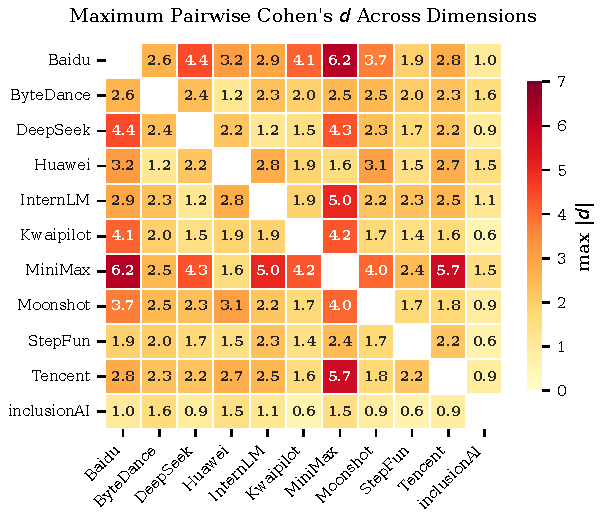
\includegraphics[width=0.50\textwidth]{figures/fig2_cohen_d_heatmap.pdf}
  \caption{Maximum pairwise Cohen's $d$ across all 8 dimensions for each model pair. All pairs exhibit at least one large effect ($d \geq 0.8$); the largest is Baidu vs.\ MiniMax ($d=6.2$ on Intuition).}
  \label{fig:cohens_d}
\end{figure}

% Figure 3: Inter-dimension correlation
\begin{figure}[t]
  \centering
  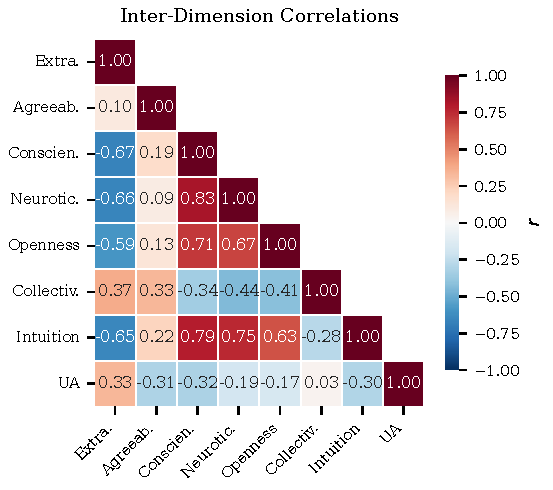
\includegraphics[width=0.40\textwidth]{figures/fig3_inter_dim_corr.pdf}
  \caption{Inter-dimension correlations at the model level ($n=33$). The strong C--N correlation ($r=0.83$) reflects acquiescence bias rather than a substantive construct relationship (PC1 explains 52\% of variance).}
  \label{fig:corr}
\end{figure}

% Figure 4: Study 2 trajectories
\begin{figure*}[t]
  \centering
  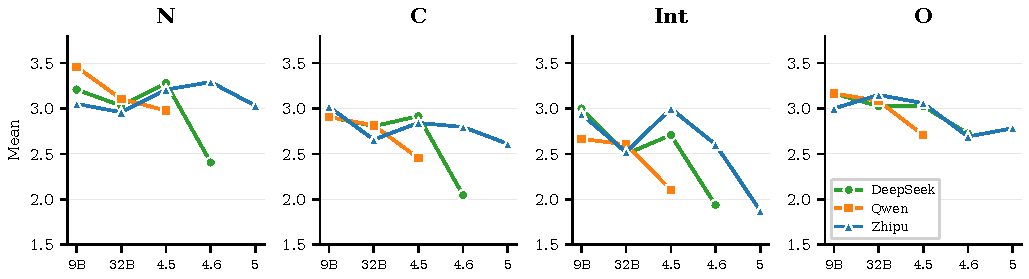
\includegraphics[width=0.85\textwidth]{figures/fig4_study2_trajectories.pdf}
  \caption{Within-model response style trajectories across model versions for DeepSeek (V2.5$\rightarrow$R1), Qwen (4B$\rightarrow$397B), and Zhipu (GLM-4$\rightarrow$GLM-5). Each panel shows a different psychometric dimension. Models exhibit distinct evolutionary patterns, suggesting alignment training shapes response styles over time.}
  \label{fig:trajectories}
\end{figure*}
